%%%%%%%%%%%%%%%%%%%%%%%%%%%%%%%%%%%%%%%%%%%%%%%%%%%%%%%%%%%%%%%%%%%%%%%%%%%%%%%%
%% MASTER'S THESIS                                                            %%
%%                                                                            %% 
%% Title (en): Mining Parallel Corpora from the Web                           %%
%% Title (sk): Rafinácia paralelných korpusov z webu                          %%
%%                                                                            %%
%% Author: Bc. Jakub Kúdela                                                   %%
%% Supervisor: Doc. RNDr. Irena Holubová, Ph.D.                               %%
%% Consultant: RNDr. Ondřej Bojar, Ph.D.                                      %%
%%                                                                            %%
%% Academic year: 2015/2016                                                   %%
%%%%%%%%%%%%%%%%%%%%%%%%%%%%%%%%%%%%%%%%%%%%%%%%%%%%%%%%%%%%%%%%%%%%%%%%%%%%%%%%

\chapter{Proposed Method}
\label{chapter:proposed_method}

This chapter describes our solution to the task of bilingual document alignment. The method has been already outlined in Section~\ref{section:overview_of_proposed_method} of Chapter~\ref{chapter:background_work_and_prerequisities} containing an introduction to all the resources and tools used in our work. The following text discusses our method in a greater level of detail.

\section{Task Definition}
\label{section:task_definition}

Our method solves an extended version of the bilingual document alignment task. This version of the task can be defined as follows: let us assume we have a number of sets containing documents from both the languages of our interest. We call these sets \textit{bins}. Each bin represents a stand-alone set of input documents for the original task. The solution of this task is a collection of pairs of documents where each pair consists of two parallel documents from the same bin.

A bin can contain up to millions of documents and is not required to have a balanced language distribution. Individual bins may vary in size. The method does not align the documents either belonging to the different bins or having the same language. Intuitively, the smaller the size of bin, the better the quality of the resulting alignment. It also takes more time and memory to align a larger bin.

When mining bilingual parallel corpora from the web, one can form a bin for every identified bilingual web domain. Such a bin can contain all the paragraphs in both the languages, scraped from the domain. This way the method will consider aligning of all the paragraphs from the domain regardless of the URLs and HTML structures of its web pages.

\section{Training Part I: Dictionary, Word Vectors}
\label{section:method_training_1}

Our method is supervised and needs to be trained on an already existing sentence-aligned corpus for the language pair we are interested in. For better clarity, we distinguish between two parts of the training process. This section describes the first part of training, while the other part is described in Section~\ref{section:method_training_2}. When trained, Section~\ref{section:method_running} explains how the method aligns the input data.

Let us describe the first part of the training process as depicted in Figure~\ref{figure:method_1}. Within the diagram, rectangles represent data in various formats, ovals stand for processing steps and arrows symbolize the flow of the process. The objective of this part of the training, is to preprocess the training parallel corpus and create a bilingual dictionary together with bilingual word vectors. The process is described in the following text.

\begin{figure}[!htb]
	\centering
	\caption{Proposed method: training part I}
	\label{figure:method_1}
	\vspace{1em}
	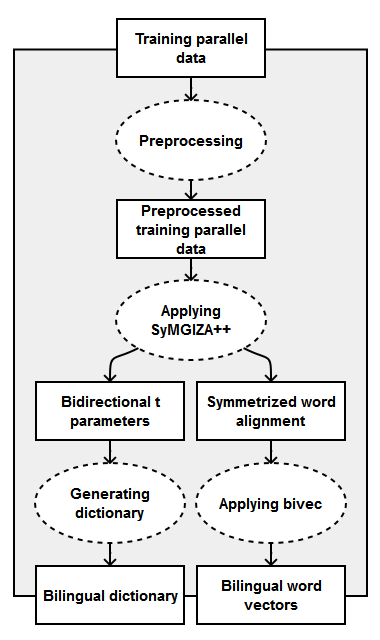
\includegraphics[width=0.50\textwidth]{images/method_1.png}
\end{figure}

\subsection{Preprocessing Training Parallel Data}
\label{subsection:preprocessing_training_parallel_data}

The procedure begins with preprocessing of the sentence-aligned training parallel corpus which may involve tokenization, lemmatization, stemming, truecasing, lowercasing, removing unknown symbols, removing stop words, etc. For individual language pairs, different preprocessing steps might help to gain better quality results. Any type of preprocessing done in this step needs be also applied to the input data, before the alignment process starts, for the method to work properly. However, this does not mean, that the user must end up with pairs of parallel documents in preprocessed format. The method is easily extensible to be able to track down the original documents. 

In our experiments with Czech--English language pair, the preprocessing includes either tokenization or lemmatization, followed by lowercasing. The tokenization and lemmatization is done utilizing MorphoDiTa (see Section~\ref{section:morphodita}), an open-source morphological dictionary and tagger.
	
\subsection{Applying SyMGIZA++}
\label{subsection:applying_symgiza}

The method follows the well-known recommendations to get a good-quality word alignment. The resulting corpus from the previous step is further cleaned by removing all the sentence pairs, where one of the sentences contains more than $50$ tokens or does not contain a single letter from any alphabet.

Then SyMGIZA++ (see Section~\ref{section:symgiza}) is executed to obtain the word alignment for the preprocessed and cleaned training parallel corpus. This step includes preparation of word classes and word co-occurrences which are used in the alignment process. The results of the execution include the values of the IBM Model 1 ``t'' parameters, after its last iteration, for both directions.

\subsection{Generating Dictionary}
\label{subsection:generating_dictionary}

The bilingual dictionary is built using the final IBM Model ``t'' parameters estimated by SyMGIZA++. The algorithm is the same as the one implemented in Bitextor's script for creating a custom dictionary (see Section~\ref{section:bitextor}). Each word pair that appears in both directions and has the harmonic mean of the ``t'' parameters (i.e.\ \textit{weight}) great enough, is included into the dictionary. Unlike the Bitextor's one, this type of a dictionary includes also the weights.

We created a script \texttt{merge\_param.py} which takes the SyMGIZA++ vocabulary files for both languages, files containing ``t'' parameters for both directions, a threshold for the weights and produces a bilingual dictionary. Listing~\ref{listing:train_dictionary} shows a sample from the file containing bilingual dictionary created by this script.

\begin{lstlisting}[float=!htb,caption={Sample from a file with bilingual dictionary (training)},label={listing:train_dictionary},firstnumber=170724]
řekl	said	0.448062
řekl	told	0.162753
řekl	say		0.0364408
řekl	tell	0.0109902
\end{lstlisting}

By default, we keep all the pairs of words with weight more than $0.00001$. The threshold is set relatively low, producing large dictionaries. Searching through a larger dictionary takes more memory and computational time which heavily affects the overall performance of the method. The reasoning behind such a low threshold is that we wanted to demonstrate the limits of our method's precision rather than its performance. Yet, we consider the chosen threshold as still acceptable when talking about the resource requirements of the method.

\subsection{Applying bivec}
\label{subsection:applying_bivec}

The input files for bivec (see Section~\ref{section:bivec}) training are obtained by vertically splitting SymGIZA++ output file \texttt{all.A3.final\_symal}. Each line of this file contains a pair of parallel sentences along with their word alignment in a format introduced by Pharaoh\footnote{\url{http://www.isi.edu/licensed-sw/pharaoh/} (accessed May 2, 2016)}, a machine translation decoder. 

It is worth noting that bivec was built to accept alignment format of Berkeley Aligner\footnote{\url{https://code.google.com/archive/p/berkeleyaligner/} (accessed April 13, 2016)}, which is another word alignment tool. To transform the Pharaoh format into the required one, all the dashes must be replaced with spaces.

The method follows the recommendations of how should be the training data preprocessed. All the sequences of numbers are replaced with a zero symbol and all the unknown symbols (e.g.\ non-printable Unicode characters) with the specially dedicated tag \texttt{<unk>}.

With all the input files for training prepared, bivec is executed to create the bilingual word vectors. It is set to generate vectors with $40$ dimensions. Listing~\ref{listing:train_bivec_cs} and Listing~\ref{listing:train_bivec_en} show samples taken from the files containing bilingual word vectors produced by bivec. Additionally, Table~\ref{table:bivec_word_similarities} lists a sample of cosine similarities between the word vectors. In the table, the order of the Czech and English words is the same, so the diagonal represents translations.

There is a reason, why we keep the number of dimensions relatively low. The word vectors are used to calculate the aggregate document vectors with the same number of dimensions. The document vectors are then indexed using Annoy (see Section~\ref{section:annoy}). The authors of Annoy suggest that the tool works best with number of dimensions less than $100$. On the other hand, the authors of bivec conducted the tests using $40$, $128$, $256$ and $512$ dimensions. We have decided to use the only number of dimensions suitable for Annoy that has been tested.

\begin{lstlisting}[float=!htb,caption={Sample from a file with Czech word vectors (training)},label={listing:train_bivec_cs},firstnumber=89]
řekl 0.610664 0.186801 0.586637 -0.305300 0.785947 -0.114462 -0.168189 -0.800271 0.761297 -0.286534 0.195719 -0.125131 -0.821144 0.049325 -0.603093 -0.183007 0.240985 0.083267 0.144988 -0.375526 0.269821 -0.266884 0.141238 0.163624 -0.385829 0.255967 -0.700835 0.451331 0.341263 0.333853 0.177087 -0.085332 -0.222975 0.753013 0.005252 0.023802 -0.520247 -0.062342 -0.485972 -0.216207
\end{lstlisting}

\begin{lstlisting}[float=!htb,caption={Sample from a file with English word vectors (training)},label={listing:train_bivec_en},firstnumber=64]
said 0.601102 0.260525 0.566347 -0.263702 0.673600 -0.114424 -0.137723 -0.704463 0.619913 -0.402364 -0.043697 -0.052677 -0.862785 0.107025 -0.665232 -0.119659 0.101142 -0.086549 -0.105953 -0.572788 0.379709 -0.309156 0.056748 0.016574 -0.131031 0.380851 -0.356606 0.340167 0.374560 0.466035 0.319632 -0.070731 -0.221821 0.630211 0.117143 0.033079 -0.416265 -0.012100 -0.469880 -0.166465
\end{lstlisting}

\begin{table}[!htb]
	\centering
	\caption{Sample of cosine similarities between word vectors}
	\label{table:bivec_word_similarities}
	\vspace{1em}
	\begin{tabular}{|c|ccccc|}
		\hline
		& \textbf{řekl} & \textbf{kočka} & \textbf{pes} & \textbf{káva} & \textbf{čaj} \\
		\hline
		\textbf{said} & \textbf{0.9522} & 0.4480 & 0.4403 & 0.4492 & 0.5440 \\
		\textbf{cat} & 0.4070 & \textbf{0.9383} & \textbf{0.8350} & 0.5053 & 0.5346 \\
		\textbf{dog} & 0.4950 & \textbf{0.7727} & \textbf{0.9328} & 0.3900 & 0.5582 \\
		\textbf{coffee} & 0.4682 & 0.4423 & 0.3880 & \textbf{0.8456} & \textbf{0.9041} \\
		\textbf{tea} & 0.5014 & 0.4202 & 0.4232 & \textbf{0.8129} & \textbf{0.9698} \\ 
		\hline
	\end{tabular}
\end{table}


\section{Training Part II: Classifier}
\label{section:method_training_2}

With the first part of the training done, the method has prepared the preprocessed training parallel corpus (see Section~\ref{subsection:preprocessing_training_parallel_data}), bilingual dictionary with weights (see Section~\ref{subsection:generating_dictionary}), and bilingual word vectors (see Section~\ref{subsection:generating_document_vectors}).

The second part of the training process is illustrated in Figure~\ref{figure:method_2}. The process is almost the same as the procedure of running the trained method. The difference is that in training, we are aligning a supervised dataset with the intention to train a binary classifier able to decide whether to accept a pair of documents as parallel or not. The trained classifier is then used when running the trained method on the input data. The following text describes the procedure of the second part of the training.

\begin{figure}[!htb]
	\centering
	\caption{Proposed method: training part II}
	\label{figure:method_2}
	\vspace{1em}
	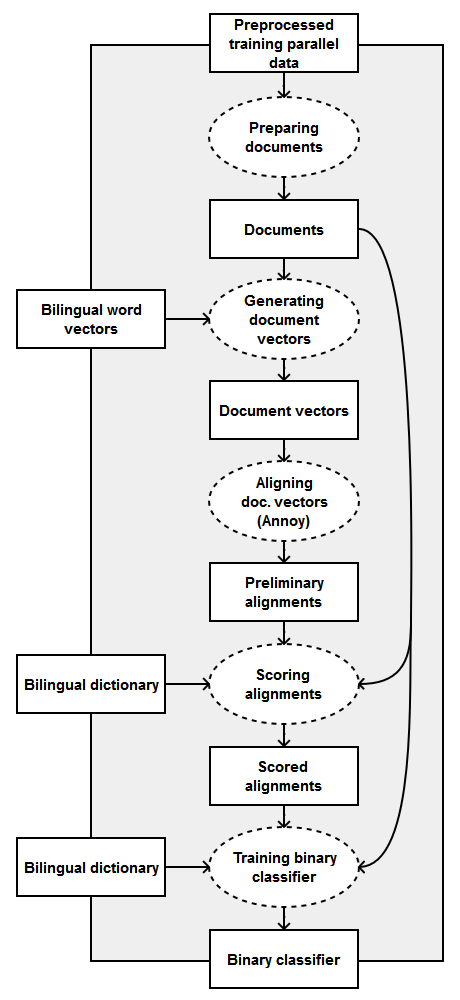
\includegraphics[width=0.60\textwidth]{images/method_2.png}
\end{figure}

\subsection{Preparing Documents}
\label{subsection:preparing_documents}

The first step creates the supervised dataset. The dataset consists of bins containing bilingual parallel documents. It is formed from the pairs of parallel sentences contained in the preprocessed training parallel corpus (see Section~\ref{subsection:preprocessing_training_parallel_data}). These are considered as pairs of parallel documents for the training.

In Section~\ref{section:task_definition}, we have explained the concept of the bins. The method splits all the pairs of documents into equally large bins (except the last one). The size of the bin should be an estimate of an expected size of the bin in a real-world dataset. In our experiment we split the documents into training bin consisting of $50,000$ pairs of parallel documents, i.e. $100,000$ documents. We consider this value as an upper-bound estimate of an average number of paragraphs in either of the two languages located on an ordinary bilingual web domain.

Our implementation accepts the supervised dataset in the form of two files, one for each language. Listing~\ref{listing:train_doc_cs} and Listing~\ref{listing:train_doc_en} show samples of such a pair of files. The format is a list of tab-separated values. The first column is an identifier of the bin. The samples show those parts of the files, where the first bin ends and the second bin starts. For the implementation to be able to iterate over both these files simultaneously, it is required that the bins are sorted in an alphabetic order. The second column is an identifier of the document. This identifier needs to be unique at least within the bin. The third column it the textual content of the document. The examples show documents from the tokenized and lowercased training parallel corpus. For the training to be successful, it is essential that each pair of parallel documents share the same bin and document identifier. This way the method knows which pairs of the documents are parallel.

\begin{lstlisting}[float=!htb,caption={Sample from a file with Czech documents (training)},label={listing:train_doc_cs},firstnumber=49999]
00000000	49998	" stál jsem támhle u zdi , " řekl .
00000000	49999	" nešpehoval jsem , harry .
00000001	50000	nikam nechodíme .
00000001	50001	pokračujte pane farbere .
\end{lstlisting}
	
\begin{lstlisting}[float=!htb,caption={Sample from a file with English documents (training)},label={listing:train_doc_en},firstnumber=49999]
00000000	49998	' i was standing there by the wall , ' he said .
00000000	49999	' i was n't spying , harry .
00000001	50000	we never socialize .
00000001	50001	continue , mr . farber .
\end{lstlisting}

\subsection{Generating Document Vectors}
\label{subsection:generating_document_vectors}

For each document, an associated vector is generated using the bilingual word vectors obtained in the first part of the training (see Section~\ref{subsection:applying_bivec}) together with the \textit{tf-idf} (term frequency-inverse document frequency) weighting scheme. The tf-idf weight of a term $d_i$ in a document $d=(d_1, d_2, \ldots,d_n)$ can be expressed as:

\begin{align*}
\operatorname{tf-idf}(d_i, d) = \operatorname{tf}(d_i, d) \times \operatorname{idf}(t) = \operatorname{tf}(d_i, d) \cdot \log \left(\frac{N}{\operatorname{df}(d_i)} \right)
\end{align*}

where $\operatorname{tf}(d_i, d)$ is the number of occurrences of the term $d_i$ in the document $d$, $\operatorname{df}(d_i)$ is the number of documents containing the term $d_i$, and $N$ is the number of all the documents in a dataset.

Our implementation processes both the files with documents one by one, bin by bin. When processing a bin, all the duplicate documents present in the bin are first discarded. Then, the inverse document frequencies are calculated for all the words that appear in the bin. Lastly, the document vector for every unique document $d=(d_1, d_2, \ldots, d_n)$ is generated as:
	
\begin{align*}
\operatorname{docvec}(d)=\sum\limits_{i=1}^{n} \operatorname{tf-idf}(d_i, d) \times \operatorname{wordvec}(d_i)
\end{align*}
	
where $\operatorname{wordvec}(d_i)$ is the word vector for the term $d_i$. The product operation in the formula is a multiplication of a scalar with a vector and the summation is derived from the operation of vector addition. If a word vector does not exist for a given term, a zero vector is used instead.
	
The described procedure is implemented in a script called \texttt{create\_docvec.py}. When given a file with documents and a file with word vectors for the associated language, it generates an output file containing document vectors. Listing~\ref{listing:train_docvec_cs} and Listing~\ref{listing:train_docvec_en} show a sample of its output. These lines contain the document vectors produced for the first pair of parallel documents displayed in Listing~\ref{listing:train_doc_cs} and Listing~\ref{listing:train_doc_en}. The output format of the script is very similar to the format of a file with documents. The only difference is that the document contents are replaced with document vectors.

\begin{lstlisting}[float=!htb,caption={Sample from a file with Czech document vectors (training)},label={listing:train_docvec_cs},firstnumber=49999]
00000000	49998	8.180257 -6.041753 6.456024 -7.385942 4.504289 -2.480280 -2.110008 -6.952853 9.294062 -5.956102 0.873277 0.288546 -8.055108 3.530353 -13.852273 1.189734 6.368119 4.307136 2.640194 -5.734687 -3.508690 -3.307812 -4.178317 -5.088661 -2.772588 10.505361 -7.485562 5.391955 5.723570 6.392571 3.516147 -1.386106 -5.184054 11.635170 -7.812555 6.185200 -0.854625 2.147744 -5.315508 1.234217
\end{lstlisting}

\begin{lstlisting}[float=!htb,caption={Sample from a file With English document vectors (training)},label={listing:train_docvec_en},firstnumber=49999]
00000000	49998	3.407737 -6.297829 7.404373 -6.480918 3.653056 0.363053 -0.486428 -4.324950 7.306768 -3.102215 -0.762884 -1.544800 -6.174080 0.820872 -10.864064 -1.982250 4.873059 -1.361170 -2.714015 -4.592477 2.429560 -1.330689 -4.640379 -3.568162 -1.444272 10.333115 -5.498119 1.396311 3.515478 9.095764 2.544416 -1.068039 -5.637783 5.594423 -3.433248 4.237183 0.336851 -0.263934 -2.851157 2.225453
\end{lstlisting}

\subsection{Aligning Document Vectors (Annoy)}
\label{subsection:aligning_document_vectors}

For each bin, the following procedure is performed. First, a search index is built containing the vectors of all the bins' documents in \textit{target language}. To build the search index, the method uses Annoy (see Section~\ref{section:annoy}) set to operate with the angular distance. Then, for every bin's document in the \textit{source language}, the index is searched to obtain $k$-approximate-nearest-neighbours to its vector. This returns a list of candidate parallel documents in the target language to the document in the source language. We call these preliminary alignments.

This procedure is implemented in a script called \texttt{align\_docvec.py}. When given files with the document vectors for both the languages, it creates an output file containing preliminary alignments. Listing~\ref{listing:train_align} shows a sample of its output. The first column is the bin identifier. The second and the third columns represent the identifiers of the documents in the source and the target language, respectively. The last column contains the similarity derived from the distance provided by Annoy calculated as $1-(d/2)$, where $d$ is the returned angular distance explained to be actually a Euclidean distance of normalized vectors. In the case presented in the sample, the parallel document ended as the 9\textsuperscript{th} best candidate (see line 4573319 in Listing~\ref{listing:train_align}).

\begin{lstlisting}[float=!htb,caption={Sample from a file with preliminary alignments (training)},label={listing:train_align},firstnumber=457311]
00000000	49998	44560	0.800532951951
00000000	49998	11723	0.791310846806
00000000	49998	9227	0.787315234542
00000000	49998	33875	0.781678438187
00000000	49998	18861	0.779217585921
00000000	49998	24646	0.771993637085
00000000	49998	9232	0.771212115884
00000000	49998	48420	0.770708605647
00000000	49998	49998	0.770486533642
00000000	49998	20284	0.768467396498
\end{lstlisting}

\subsection{Scoring Alignments}
\label{subsection:scoring_alignments}

Within the preliminary alignments, the top candidates are not necessarily the optimal ones. Therefore, the method applies a scoring function to reorder the candidates. This increases the probability of the optimal documents to appear higher in their candidate lists. Given the document $d=(d_1, d_2, \ldots,d_n)$ and its candidate $c=(c_1, c_2, \ldots, c_m)$, the scoring function is defined as:
	
\begin{align*}
\operatorname{score}(d, c)=\operatorname{length\_sim}(d, c) \times \operatorname{weight\_sim}(d, c)
\end{align*}
	
Both the functions $\operatorname{length\_sim}(d, c)$ and $\operatorname{weight\_sim}(d, c)$ have the range of $[0, 1]$. The idea is that the higher the result they return, the greater the possibility that the pair is parallel. These functions are defined as follows.

\begin{itemize}
	\item $\operatorname{length\_sim}(d, c)$ examines the ratio of the documents' lengths. It is based on the probability density function of the normal (Gaussian) distribution:
	
	\begin{align*}
	\operatorname{length\_sim}(d, c)=e^{-\dfrac{(\frac{\operatorname{len}(c)}{\operatorname{len}(d)}-\mu)^2}{2\sigma^2}}
	\end{align*}
	
	where $\frac{\operatorname{len}(c)}{\operatorname{len}(d)}$ is the actual ratio of the documents' lengths and $\mu$ is the expected ratio with the standard deviation $\sigma$. The expected ratio of documents's lengths with the associated standard deviation can be estimated using the pairs of parallel sentences from the preprocessed training parallel corpus. For the tokenized Czech--English parallel corpus these values are estimated to be $\mu_{cs \rightarrow en} \approx 1.08$ and $\sigma_{cs \rightarrow en} \approx 0.28$.
	
	\item $\operatorname{weight\_sim}(d, c)$ is based on the IBM Model 1~\cite{Brown93} and uses the bilingual dictionary created in the first part of the training. It is defined as:
	
	\begin{align*}
	\operatorname{weight\_sim}(d, c)=\prod\limits_{i=1}^{n} \sum\limits_{j=1}^{m} \frac{\operatorname{weight}(d_i, c_j)}{m}
	\end{align*}
	
	where $\operatorname{weight}(d_i, c_j)$ is the weight of the word pair $\langle d_i,c_j \rangle$ provided by the dictionary if the entry exists, otherwise it equals $10^{-9}$ (``null weight'').
\end{itemize}

A script called \texttt{score\_align.py} implements the described procedure. Given a file with preliminary alignments and files with the documents for both the languages, it creates an output file containing scored alignments. Listing~\ref{listing:train_score} shows a sample of its output. The output format is almost unchanged when compared with the format of a file with preliminary alignments. The only difference is that the similarity in the last column is replaced with the calculated score. The presented sample shows scored candidates from Listing~\ref{listing:train_align}. The matching document is now considered as the top candidate.

\begin{lstlisting}[float=!htb,caption={Sample from a file with scored alignments (training)},label={listing:train_score},firstnumber=457311]
00000000	49998	49998	1.21903368318e-14
00000000	49998	20284	9.19687934061e-20
00000000	49998	11723	1.55923045256e-23
00000000	49998	9232	9.73231577325e-25
00000000	49998	18861	7.95893854924e-27
00000000	49998	48420	8.82180461894e-28
00000000	49998	33875	1.19519536122e-30
00000000	49998	9227	1.70133029025e-38
00000000	49998	44560	2.16354386116e-43
00000000	49998	24646	9.5437947187e-55
\end{lstlisting}

\subsection{Training Binary Classifier}
\label{subsection:training_binary_classifier}

It is required from the binary classifier to be able to decide whether to accept a pair of documents as parallel or not. The chosen model for the classifier is a feed-forward neural network~\cite{Sima96}. The method uses an implementation provided by PyBrain (see Section~\ref{section:pybrain}). The classification is based on 4 features. All of these features have the range of $[0, 1]$. Given the document $d=(d_1, d_2, \ldots, d_n)$ and its candidate $c=(c_1, c_2, \ldots, c_m)$, the following list describes all the features.

\begin{itemize}
	\item $\operatorname{length\_sim}(d, c)$ has been already defined (see Section~\ref{subsection:scoring_alignments}). This function scores the ratio of the documents' lengths against the expected ratio.

	\item $\operatorname{length\_conf}(d, c)$ provides a supplementary information for the previous feature, which is not a reliable nor effective when scoring pairs of short documents; however, it is substantial when comparing pairs of long documents:
		
	\begin{align*}
	\operatorname{length\_conf}(d, c)=1 - e^{-0.01 \times \operatorname{len}(d)}
	\end{align*}
		
	This is a monotonically increasing function, that provides the model with an information of absolute length of the document $d$. The name of the feature is an abbreviation of ``length confidence'', which is justified by the fact that the higher the value of the $\operatorname{length\_conf}(d, c)$ is, the more authoritative is the score of the $\operatorname{length\_sim}(d, c)$.
		
	\item $\operatorname{weight\_sim_2}(d_i, c_j)$ is a modified version of $\operatorname{weight\_sim}(d, c)$ (see Section~\ref{subsection:scoring_alignments}). The original version was tested for the purposes of the classification, but the results were poor. This might be caused by the fact, that it returns very small values affected by the number of words contained in both the documents to a large extent. The modified version is defined as:

	\begin{align*}
	\operatorname{weight\_sim_2}(d, c)=\frac{\sum\limits_{i=1}^{n} \operatorname{len}(d_i) \times \max\limits_{j=1}^{m}\left(\operatorname{weight_2}(d_i, c_j)\right)}{\sum\limits_{i=1}^{n} \operatorname{len}(d_i) \times \operatorname{sgn}(\max\limits_{j=1}^{m}\left(\operatorname{weight_2}(d_i, c_j)\right))}
	\end{align*}
		
	where $\operatorname{weight_2}(d_i, c_j)$ is defined as the weight of the word pair $\langle d_i,c_j \rangle$ provided by the dictionary if the entry exists; however, if it does not exist and the two words are identical, then it equals $1$, otherwise it returns $0$.
		
	Let us explain the reason behind the heuristic of $\operatorname{weight_2}(d_i, c_j)=1$ for a pair of identical words not having entry present in the dictionary. The same set of features is used in the running process where occurrences of new words or special terms (e.g. URLs or email addresses) are expected. The heuristic considers a pair of identical words to be a perfect translation only if the dictionary does not contain other relation.
	
	Additionally, let us discuss why the weights are multiplied by the lengths of words. The assumption is that longer words are usually less frequent, carry more meaning and are therefore more important for the sentence, in contrast to short tokens (e.g. ``,'' or ``a''). The definition of $\operatorname{weight\_sim_2}(d, c)$ is an arithmetic mean of strongest relations between a source word from $d$ and any of the target words from $c$, weighted by the lengths of source words.

	Figure~\ref{figure:weight_sim} shows an example of $\operatorname{weight\_sim_2}$ calculation. In the example, for every source word in the Czech document, there exists an entry in the bilingual language dictionary with at least one of the target words from the English candidate document. Arrows represent the strongest among the relations ($\max\operatorname{weight_2}$) for each of the source words. The calculation above each of the source words is a multiplication of the length of the source word and the weight of the associated strongest relation.
\end{itemize}
		
\begin{figure}[!htb]
	\centering
	\caption{Example $\operatorname{weight\_sim_2}$ calculation}
	\label{figure:weight_sim}
	\vspace{1em}
	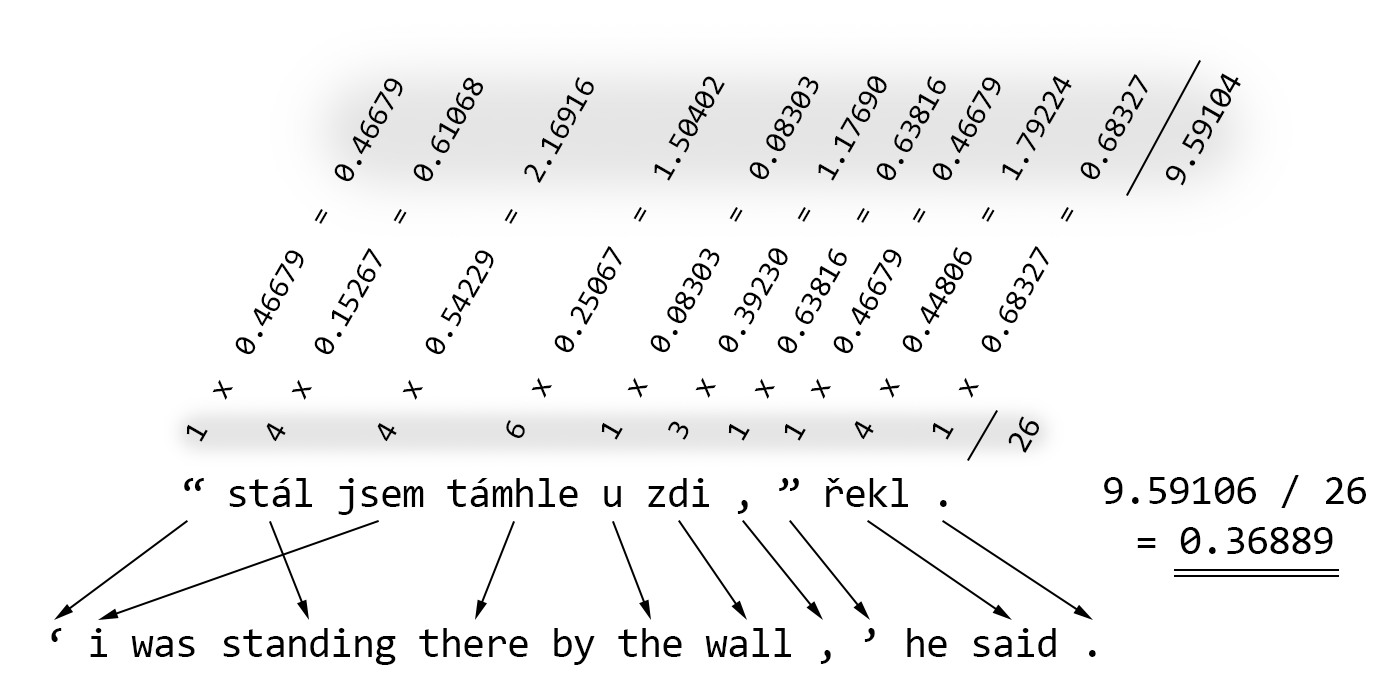
\includegraphics[width=0.8\textwidth]{images/weight_sim.png}
\end{figure}

\begin{itemize}[resume]
	\item $\operatorname{weight\_conf_2}$ is a supplementary feature for $\operatorname{weight\_sim_2}$. We can interpret the $\operatorname{weight\_sim_2}$ feature as: ``From what we know with the knowledge of possible incomplete dictionary, how likely are these two documents parallel?''. The supplementary feature can be similarly interpreted as: ``To what extent the dictionary covers the pairs of words we came across?''. The formal definition is following:
		
	\begin{align*}
	\operatorname{weight\_conf_2}(d, c)=\frac{\sum\limits_{i=1}^{n} \operatorname{len}(d_i) \times \operatorname{sgn}(\max\limits_{j=1}^{m}\left(\operatorname{weight_2}(d_i, c_j)\right))}{\sum\limits_{i=1}^{n} \operatorname{len}(d_i)}
	\end{align*}
\end{itemize}
	
With all the features designed for the classification defined, the process of training can be explained. It starts by creating a training dataset using the scored alignments. For every document $d$ in the source language and its top candidate $c$ in the target language the following pair of input$\rightarrow$output vectors is added into the training dataset:

\begin{align*}
\begin{pmatrix}
\operatorname{length\_sim}(d, c) \\
\operatorname{length\_conf}(d, c) \\
\operatorname{weight\_sim_2}(d, c) \\
\operatorname{weight\_conf_2}(d, c)
\end{pmatrix} \rightarrow \begin{cases}
\begin{pmatrix} 0 \\ 1 \end{pmatrix}, & \text{if } \langle d,c \rangle \text{ are parallel} \\\\
\begin{pmatrix} 1 \\ 0 \end{pmatrix}, & \text{otherwise.} \\
\end{cases}
\end{align*}

The input vector consists of the 4 defined features, while the output vector encodes whether the documents $\langle d,c \rangle$ are parallel or not. The first value of the output vector represents the probability of the documents to be non-parallel. The second value is complementary to the first.

Before the network is trained, the collected training dataset is subsampled to contain an approximately equal number of items representing parallel and non-parallel document pairs. This helps the network to be less affected by the ratio of parallel and non-parallel pairs. At this moment, it is also possible to reduce the size of the dataset to shorten the time it takes to complete the training.

This described procedure is implemented in a script called \texttt{train\_network.py}. When given a file with scored alignments and files with documents for both the languages, the script trains a network and stores its configuration to a disk on a requested location in the form of an XML file. This allows the method to load and use the trained network at any time. It also enables the system to distribute the trained model to other nodes.

\section{Running}
\label{section:method_running}

With the second part of the training done, the method has prepared a binary classifier able to decide whether to accept a pair of documents as parallel or not (see Section~\ref{subsection:training_binary_classifier}).

The process of running the trained method on the input data is illustrated in Figure~\ref{figure:method_3}. The resemblance between this process and the procedure of the second part of the training has been already discussed. Due to the large extent of similarity the shared parts of the process are described briefly as they have been discussed in detail in Section~\ref{section:method_training_2}.

\begin{figure}[!htb]
	\centering
	\caption{Proposed method: running}
	\label{figure:method_3}
	\vspace{1em}
	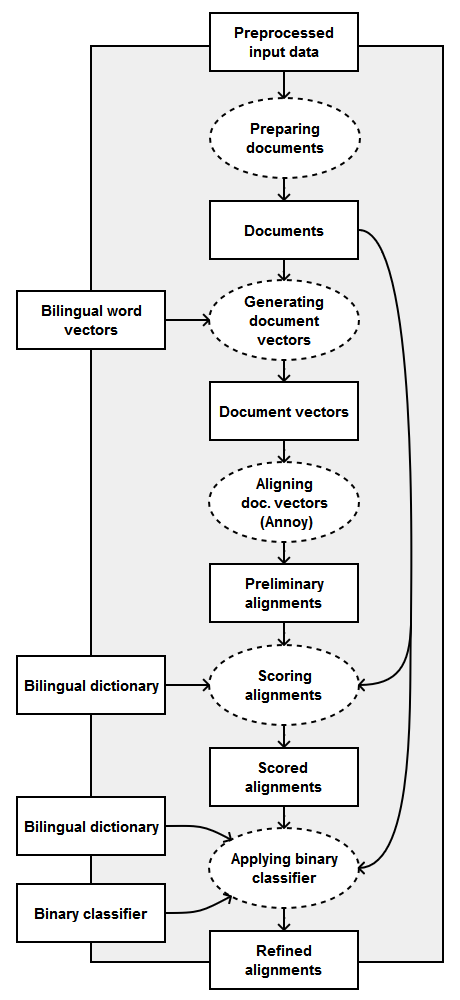
\includegraphics[width=0.60\textwidth]{images/method_3.png}
\end{figure}

\subsection{Preparing Documents}
\label{subsection:preparing_documents_running}

As mentioned earlier in Section~\ref{subsection:preprocessing_training_parallel_data}, the input documents have to be preprocessed in the same way as the training parallel corpus. Then, the preprocessed documents have to be split into bins. As already noted (see Section~\ref{section:task_definition}), when aligning paragraphs from the web, a bin can contain all the paragraphs for both the languages, scraped from one bilingual web domain. In this scenario, the names of the domains can be used as bin identifiers. This restricts the method to align only the paragraphs originating from the same domain. On the other hand, if aligning inseparable data, e.g. documents without a natural distribution into groups, all the documents can be placed into a single bin with an arbitrary identifier. However, the method has better recall when aligning smaller bins. This is caused mainly by Annoy, which has better accuracy when searching through an index with less items.

Our implementation accepts the input dataset in a form of two files, one for each language. It is the same format as for the supervised dataset, described in Section~\ref{subsection:preparing_documents}. Listing~\ref{listing:run_doc_cs} and Listing~\ref{listing:run_doc_en} show samples of such a pair of files containing Czech and English paragraphs acquired from the web.
	
\begin{lstlisting}[float=!htb,caption={Sample from a file with Czech documents (running)},label={listing:run_doc_cs},firstnumber=154290]
europa.eu	154289		v praze se fórum zaměřilo konkrétně na jadernou bezpečnost , politiky nukleárního odpadu , možné iniciativy v oblasti odborné přípravy a vzdělávání a transparentnosti .
\end{lstlisting}

\begin{lstlisting}[float=!htb,caption={Sample from a file with English documents (running)},label={listing:run_doc_en},firstnumber=1085753]
europa.eu	1085752		at the prague meeting the forum has been dedicated more particularly to nuclear safety , nuclear waste policies , possible initiatives on training and education as well as in the area of transparency .
\end{lstlisting}

\subsection{Applying Binary Classifier}
\label{subsection:applying_binary_classifier}

With the input dataset prepared, the process follows with the exact same steps applied to the supervised dataset in the second part of the training. First, vectors are generated for all the documents (see Section~\ref{subsection:generating_document_vectors}). Then, the document vectors are aligned by searching for nearest neighbours of all documents in the source language, resulting in preliminary alignments (see Section~\ref{subsection:aligning_document_vectors}) and these are subsequently scored (see Section~\ref{subsection:scoring_alignments}).

As a final step, the trained classifier (see Section~\ref{subsection:training_binary_classifier}) is used to obtain the refined alignments. For every document $d$ in the source language and its top candidate $c$ in the target language the trained network is activated as follows:

\begin{align*}
\begin{pmatrix}
\operatorname{length\_sim}(d, c) \\
\operatorname{length\_conf}(d, c) \\
\operatorname{weight\_sim_2}(d, c) \\
\operatorname{weight\_conf_2}(d, c)
\end{pmatrix} \xrightarrow{?} \begin{pmatrix} a \\ b \end{pmatrix}
\end{align*}
	
The input vector contains the same set of features as in the training. When activated, the second value from the output vector $b \in [0, 1]$ represents the confidence of a prediction that the two documents $\langle d,c \rangle$ are parallel. If the confidence $b$ is greater than a user-defined threshold, the document pair $\langle d,c \rangle$ ends up in the resulting refined alignments.

A script called \texttt{apply\_network.py} implements the described procedure. When given a file containing the network configuration of a classifier, a file with scored alignments and files with documents for both the languages, it creates an output file containing refined alignments. Listing~\ref{listing:run_refine} shows a sample of its output. The output format follows the convention of the files with preliminary and scored alignments. This time, the last column represents the confidence returned by the classifier. The presented sample shows that the two paragraphs from Listing~\ref{listing:run_doc_cs} and Listing~\ref{listing:run_doc_en} are successfully aligned.

\begin{lstlisting}[float=!htb,caption={Sample from a file with refined alignments (running)},label={listing:run_refine},firstnumber=33683]
europa.eu	154289	1085752		0.9996949388
europa.eu	154287	1085750		0.999479551945
europa.eu	154284	1163960		0.996325842675
europa.eu	154285	1163962		0.996881020525
\end{lstlisting}
\section{Discussion}
\label{section:method_discussion}

The second part of the training process and its resemblance to the procedure of running the trained method may seem cumbersome. However, in case of presence of a different binary classifier able to tell whether the two documents are parallel or not, the whole second part of the training could be excluded and the provided classifier would be utilized.

An alternative classifier could be based on a pre-trained SMT system that would be used to translate the document in the source language into the target one to be compared with the other document. This idea was adapted in the related project focused on mining Wikipedia (see Section~\ref{section:mining_wikipedia}).

Our classifier is more similar to the one used by STRAND (see Section~\ref{section:strand}). The STRAND's classifier is based on a decision tree built over a set of features comparing the similarity between a pair of potentially parallel HTML structures. In contrast to this, our method uses a neural network trained with a set of features designed to compare two potentially parallel plain text documents.

In our method, the second part of the training process simulates the aligning of a supervised dataset with the knowledge of the optimal solution. In the end of the procedure, the model of the classifer is trained. This is a generic approach that can be easily modified. One can redesign the set of features for the classification or completely change the implementation of the learning model.

Inspired by STRAND's classifier, we tried to swap the neural network model with a model based on a decision tree using the same set of features. For these purposes, we used the implementation provided by Scikit-learn~\cite{Pedregosa11}, a Python machine learning library. The tentative results were poorer; however, we did not spend that much time with trying different parameters and testing.

It is important to note, that the method, in its present form, does not take into account the order of the words when aligning parallel documents. The tf-idf weighting scheme, the scoring function based on the IBM Model 1 and even all the features used by the classifier completely ignore this aspect. Despite the fact that the results are promising, there are places for improvement.

It is also important to highlight the fact that our method is asymmetric regarding the fact that it generates different results if the source and the target languages are swapped. The main reason behind this is that the document vectors associated with the target language are indexed by Annoy while the other vectors for the source language are used as query points for the approximate-nearest-neighbours search. From our experience, a rule of thumb is to choose the language with more documents to be the target one.

The method is designed to be able to run in parallel or distributed environment. Bins with input documents represent independent isolable tasks. These can be distributed across multiple nodes together with the once trained resources needed for the execution. These include bilingual dictionary, bilingual word vectors and the trained classifier.

The key idea behind our method is to use the combination of bilingual word embedding and locality-sensitive hashing. Usually the most expensive operation when solving the task of document alignment is the content comparison of the two documents. A naive approach compares each of the $N$ documents in the source language, with all the $M$ documents in the target language resulting in $N \times M$ comparisons. Our method reduces this number to $N \times k + N$. The $N \times k$ is the number of comparisons needed for the scoring of the $k$ candidates from all the possible $M$ ones as returned by the approximate-nearest-neighbours search and $N$ is the number of comparisons necessary for the final classification of the top candidates.